\documentclass[12pt]{report}
\usepackage[]{graphicx}\usepackage[]{color}
%% maxwidth is the original width if it is less than linewidth
%% otherwise use linewidth (to make sure the graphics do not exceed the margin)
\makeatletter
\def\maxwidth{ %
  \ifdim\Gin@nat@width>\linewidth
    \linewidth
  \else
    \Gin@nat@width
  \fi
}
\makeatother

\definecolor{fgcolor}{rgb}{0.345, 0.345, 0.345}
\newcommand{\hlnum}[1]{\textcolor[rgb]{0.686,0.059,0.569}{#1}}%
\newcommand{\hlstr}[1]{\textcolor[rgb]{0.192,0.494,0.8}{#1}}%
\newcommand{\hlcom}[1]{\textcolor[rgb]{0.678,0.584,0.686}{\textit{#1}}}%
\newcommand{\hlopt}[1]{\textcolor[rgb]{0,0,0}{#1}}%
\newcommand{\hlstd}[1]{\textcolor[rgb]{0.345,0.345,0.345}{#1}}%
\newcommand{\hlkwa}[1]{\textcolor[rgb]{0.161,0.373,0.58}{\textbf{#1}}}%
\newcommand{\hlkwb}[1]{\textcolor[rgb]{0.69,0.353,0.396}{#1}}%
\newcommand{\hlkwc}[1]{\textcolor[rgb]{0.333,0.667,0.333}{#1}}%
\newcommand{\hlkwd}[1]{\textcolor[rgb]{0.737,0.353,0.396}{\textbf{#1}}}%

\usepackage{framed}
\makeatletter
\newenvironment{kframe}{%
 \def\at@end@of@kframe{}%
 \ifinner\ifhmode%
  \def\at@end@of@kframe{\end{minipage}}%
  \begin{minipage}{\columnwidth}%
 \fi\fi%
 \def\FrameCommand##1{\hskip\@totalleftmargin \hskip-\fboxsep
 \colorbox{shadecolor}{##1}\hskip-\fboxsep
     % There is no \\@totalrightmargin, so:
     \hskip-\linewidth \hskip-\@totalleftmargin \hskip\columnwidth}%
 \MakeFramed {\advance\hsize-\width
   \@totalleftmargin\z@ \linewidth\hsize
   \@setminipage}}%
 {\par\unskip\endMakeFramed%
 \at@end@of@kframe}
\makeatother

\definecolor{shadecolor}{rgb}{.97, .97, .97}
\definecolor{messagecolor}{rgb}{0, 0, 0}
\definecolor{warningcolor}{rgb}{1, 0, 1}
\definecolor{errorcolor}{rgb}{1, 0, 0}
\newenvironment{knitrout}{}{} % an empty environment to be redefined in TeX

\usepackage{alltt}
\newcommand{\SweaveOpts}[1]{}  % do not interfere with LaTeX
\newcommand{\SweaveInput}[1]{} % because they are not real TeX commands
\newcommand{\Sexpr}[1]{}       % will only be parsed by R



\usepackage{/home/randy/thesis/chapters/thesis}
\usepackage{pdflscape}
\usepackage{rotating}
\usepackage{setspace}
\usepackage[titles]{tocloft}
\renewcommand\cfttoctitlefont{\normalsize}
\setlength\cftchapindent{0pt}
\usepackage{fancyhdr}
\pagestyle{fancy}
\fancyhf{}
\cfoot{\thepage}
\fancyhead[R]{}
\renewcommand{\headrulewidth}{0pt}

%\usepackage[]{layout}
\usepackage[font=scriptsize]{caption}

\AtEveryBibitem{\clearfield{note}}    % clears notes

\makeatletter
\newcommand\iraggedright{%
	\let\\\@centercr\@rightskip\@flushglue \rightskip\@rightskip
	\leftskip\z@skip}
\makeatother

\usepackage{titlesec}
\titlespacing*{\chapter}{0pt}{2in}{0pt}
\titleformat{\chapter}[display]{\normalfont}{\chaptertitlename\ \thechapter}{12pt}{\normalfont}
\titleformat*{\section}{\normalsize\bfseries} 
\titleformat*{\subsection}{\normalsize\itshape} 
\titlespacing*{\section}{0pt}{0ex plus 1ex minus .2ex}{0ex plus .2ex} 
\titlespacing*{\subsection}{0pt}{0ex plus 1ex minus .2ex}{0ex plus .2ex}

\renewcommand{\chaptername}{{CHAPTER}}

\title{Cracks in the foundation: The myth of Latin American national literatures}





\begin{document}


%\begin{singlespace}
%	\setcounter{chapter}{1}
%\chapter{SPANISH NATIONALISM IN GALDÓS}
%\end{singlespace}

A re-examination of the literature of the 19th century may at first glance may appear redundant given the quantity of analysis it has already received. 
However, even without the application of new analytical techniques, Alda Blanco argues that there still exists a need for a renewed approach to the mid-nineteenth century in traditional scholarship \cite[423]{Blanco2000}.
Of particular interest is Blanco's view that the privileging of \enquote{Realism} by critics has obfuscated the reading of this period \cite[433]{Blanco2000}.
The idea that artificial classifications of genre may hinder subjective analysis is not new.
Critics such as Ted Underwood have made quantification of the effects of genre distinction central to the digital analysis of large corpora of literature. 

In \enquote{Understanding Genre in a Collection of a Million Volumes} Underwood explores an algorithmic approach to genre classification. 
At first, this appears to risk solidifying the same approach to categorization that has lead to the \enquote{missed discoveries} discussed by Blanco.
It is to strong say that genre divisions have been historically arbitrary, yet they do miss nuanced classifications, which Underwood refers to as \enquote{fuzzy boundaries} \cite[9]{Underwood2014}.
He states the strength of statistical models in genre classification is that \enquote{by characterizing and instance's mixed membership in multiple classes, or by predicting its likelihood of membership in a single class as a continuous variable} \cite[9]{Underwood2014}.
This can be seen in the previous examination of \textit{María}.
While many critics discussed the \enquote{realistic} characteristics of the novel, none classified it as \enquote{Realism}.
A more nuanced approach, aided by algorithmic classification, helps to soften the edges of the time periods often imposed on genre, potentially uncovering previously missed periods such as the 1850-1870 era of the Spanish novel explored by Blanco.

According to his investigation, it is the artificial temporal boundaries between the two \enquote{great canonical traditions of the century} that have caused critics to overlook the value of narratives in this period (425)\nocite{Blanco2000}.
Blanco argues that by placing works from mid-century into lesser categories such as \textit{costumbrista} or \textit{novelas por entregas}, critics further undermine objective investigation through the imposition of an artificial taxonomy (426)\nocite{Blanco2000}.
For this reason Underwood applies Thomas Vanderwal's moniker \enquote{folksonomy} to his classification in order to highlight the bottom up approach to the division of textual characteristics \cite{Underwood2014, Vanderwal2007}.

Sereni points out that this historical period saw the formation of of new social frameworks that re-examined not only new relationships between ownership and production but also linguistically, culturally, politically and morally \cite[Sereni in][429]{Blanco2000}.
Both authors highlight the view at the time that literature was an unstoppable cultural force viewed as possessing the ability to shape the morals of society. 
According to Blanco, in Spain this brought into question the very idea of morality itself (429)\nocite{Blanco2000}.
Nocedal furthermore insists ,that the novel be verisimilar, particularly in relationship to the two categories which he considers to be the most
problematic and dangerous in the novelistic text: the representation of gender and class relations \cite[430]{Blanco2000}.
Nocedal demands that novelistic verisimilitude be the representation of that which is “naturally” complementary between the sexes and among the social classes. 
Therefore he argues that the novel should not depict gender and class relationships as conflict or struggle \cite[430]{Blanco2000}.

Benito Pérez Galdós was one of the most prolific writers in 19th century Spain. 
Part of his literary production consists of the series of 46 novels written between 1872 and 1912 known as \textit{Los episodios nacionales}.
The works are divided up into five series with common themes and protagonists creating a historical continuum that chronicles Spanish history from 1805 to 1868.
The first novel in this series, \textit{Trafalgar}, is narrated by Gabriel Araceli.
The narrator presents himself in the beginning of the novel as an old man reflecting on his youth.
Gabriel has come to live with Don Alonso Gutiérrez de Cisniega and his wife Doña Francisca after the death of his mother.
Don Alonso and Doña Francisca have a daughter of their own who is engaged to a young soldier named Malespina.

\enquote{by focusing on defeat in the \textit{Episodios}, Galdós attempts to avert the threat of dissolution of Spanish unity} \cite[12]{Kempen2007}

According to Micheal Iarocci \textit{Trafalgar} is the most edited, read and analysed of Galdós' historical novels (183)\nocite{Iarocci2003}.
Yet he goes on to observe \enquote{if one turns to critical appraisals of the work for indications of the qualities that presumably have accorded \textit{Trafalgar} its privileged standing, one finds that the tacit assertions of superior aesthetic value that might be expected are curiously absent} \cite[183]{Iarocci2003}.


\enquote{Galdós revitalizó y revolucionó al lector español, hasta entonces acostumbrado a folletines y malas traducciones} \cite[1525]{Urey1992}

Dice en cuanta al Marcial \enquote{su lenguaje es <<mareante>> en su confusión constante de términos y definiciones} \cite[1526]{Urey1992}

\enquote{establece uno de los muchos paralelos importantes a Gabriel, que, como varios críticos han observado, es una figura picaresca, y que, a su edad, tampoco es todo un hombre} \cite[1526]{Urey1992}
This helps to highlight a tendency, as the 19th century wore on, for authors from the various new republics to depend less on the repetition of old styles and tropes.
This emphasis in a stylistic separation from their colonial past comes to fruition with the contribution of \textit{modernismo} as the first movement attributed with originating in an ex-Spanish colony.

Urey points out that Gabriel's role as narrator and character narrated put emphasis on the metafictional role of \textit{Trafalgar} \cite[1526]{Urey1992}.
Another parallel between the work of Isaacs and Galdós' \textit{Trafalgar} is the prominence of description, which Urey points intentionally puts emphasis \enquote{al acto de representar que al mundo representado} \cite[1527]{Urey1992}.


An observation unique to \textit{Trafalgar} is that individual characters serve as metaphors for particular time periods in Spain's history \cite[1527]{Urey1992}. 


As mentioned in Chapter 2, Galdós makes explicit commentary on the role of language as an identifying characteristic.
Sieber demonstrates that the connection of language, be it fictional or not, and identity has long been a component of literature \nocite{Sieber1978}(...).
The narrator in \textit{Trafalgar} says of Marcial \enquote{usaba un vocabulario formado por los más peregrinos terminachos, pues es costumbre en la gente de mar de todos los países desfigurar la lengua patria hasta convertirla en caricatura} \cite[21]{Galdós1882}.
Of particular interest is a passage examined by Ulrey in which Gabriel explains the meaning of many of Marcial's phrases.
What this highlights for the my purpose here is that this \enquote{inter-language}, not a dialect nor a language of its own, still possesses enough characteristics to merit clarification.
For Galdós, and many others, these language variations often evidenced a persons class or origin.


Within the new republics of the former Spanish empire many authors used these identifying characteristics not only to distinguish them from their colonizers, but also in order to avoid being perceived as culturally homogeneous with their neighboring regions and states.
Urey goes so far as to draw a striking parallel, noting that \enquote{al final de la Serie Gabriel [...] ha aprendido a controlar el juego de lenguaje que constituye su texto} which she claims reflects Spain's ability to recapture it's own national identity \cite[1532]{Urey}.
Iarocci points out that even the conception of the starting point for the \textit{episodios nacionales} has is origins in Galdós' awareness of the subconscious workings of language.
Galdós is quoted saying \enquote{cuando me preguntó en qué época pensaba iniciar la serie, brotó de mis labios como una obsesión del pensamiento, la palabra Trafalgar} \cite[184]{Iarocci2003}.
He elaborates that the emphasis on the word, by making it the subject of \textit{brotó}, puts the writer in the background, highlighting the importance of language in his project.


Urey states \enquote{el lenguaje puede sugerir un significado por medio de las relaciones entre palabras asociadas} \cite[1529]{Urey}.
In her case, this supports the idea that Marcial's use of language, particularly applying nautical terms to unconventional signifieds, 
Vessey's discussion of borrowing's can be applied to this scenario even though Marcial is re-appropriating words from his own language.
Choosing a signifier other than one that would be expected by the receiver can serve only one purpose which is to alter the cultural connotation associated with the word.
In the ex-colonial case these \enquote{core borrowings} frequently come from indigenous languages.
In Spain, foreign borrowing is more commonly associated with the Baroque period.
However, the parallel to inter-language borrowing is quite clear given the original of many of these \textit{culitsmos} was the mother language of Spanish, Latin.
The very term \textit{cultismo} helps to highlight the historical precedent of altering word usage in order to establish social distinction.


This establishes an historical cycle, one that David Pharies also attributes to social prestige.
He notes that linguistic changes can be initiated when one social group feels that their identity within a larger community is threatened \cite[15]{Davies2007}.
According to Pharies, who bases his discussion on theories proposed by William Labov, certain linguistic changes help distinguish those that share values and beliefs (15)\nocite{Pharies2007}.
Davies adds that \enquote{el grupo emplea una distinción lingüísica para enfatizar una distinción social} \cite[17]{Pharies2007}.
According to Clare Mar-Molinero, beyond linguistic analysis, the identifying power of language is the only explanation for the effort that humans put into maintaining thousands of mutually incomprehensible modes of communication \cite[2]{Molinero2005}.
She claims that \enquote{the answer must lie in an innate need and desire to protect difference across groups and communities} \cite[2]{Molinero2005}.
Mar-Molinero goes on to clarify that \enquote{few if any marked-out states are naturally monocultural} later noting that the attempt to usurp this cultural diversity in the nineteenth century \enquote{laid the seeds for many explosive separatist movements} \cite[10]{Molinero2005}.


Anderson acknowledges the phenomenon of linguistic social identification, but he stops short of granting regional dialects a role in the imagining of nations.
In fact, he attributes the success of print culture precisely to the homogenization of language.
He asserts that \enquote{had print capitalism sought to exploit each potential oral vernacular market, it would have remained a capitalism of petty proportions} and continues \enquote{these idiolects were capable of being assembled, within definite limits, into print-languages far fewer in number} \cite[43]{Anderson2006}.
There is no doubt that this was a conscious undertaking on the part of the newly independent states.
However, the stylistic features that distinguish the novels examined here can be seen as being used to create the social distinction that Pharies talks about.
In the former Spanish colonies this distinction helps to reinforce geographic political boundaries.
In Anderson's study these developing communities of nation must be geographically limited.
Because the borders throughout the Spanish colonies were evolving throughout the 19th century, language was an especially powerful way to link one's identity to one's territory.
The admission into popular readings of a growing number of indigenous borrowing and regional colloquialisms served as an important means to create identity within a largely homologous umbrella of inherited colonial language.

Both Isaac's and Galdós were writing about similar socio-political struggles although choosing to treat them in very divergent ways.
In Eamonn Rodgers' words \enquote{the expulsion of the French from the Peninsula in 1813, had created the image of a fiercely independent people, heroically defending their land and their liberty against a tyrant} \cite[465]{Rodgers2005}.
Despite their drastically different histories, the timeline for re-defining national identitiy is very similar.
As Iarocci asserts \enquote{the story of modern Spain continues to begin somewhere within the vicinity of the War of Independence (1808-1814)} \cite[185]{Iarocci2003}.
Iarocci also points out the importance of not only viewing this as a \enquote{history} but also the \textit{bildungsroman} of Gabriel Araceli \cite[189]{Iarocci2003}.
Seen as a novel of formation, the love allegories of Latin America appear more closely relatable to Galdós' work.
He concludes that \enquote{an analysis of the interconnections between the sentimental and historical plots} helps reveal \enquote{the preoccupation with the social status and meaning of masculinity} \cite[190]{Iarocci2003}.

Chapter 1 explored how Sommer connects nationalism and novel in Latin America through the allegory of frustrated eroticism and \enquote{ideal gender models that were teaching future republicans to be passionate in a rational and seductively horizontal way} \cite[191]{Iarocci2003}. 
\textit{Trafalgar} explores the evolution of gender in Spain.
According to Iarocci, Galdós' version of history serves to question the \enquote{cultural ideal of heroic masculiity} \cite[191]{Iarocci2003}.
The directness of Galdós' treatment is apparent from the outset in the emasculating description of Marcial's aged existence.
This parallel between participating in history, charging off to battle, and the journey to manhood mirrors \enquote{the assumption of an adult male gender identity on one hand, and the emergence of a nationalist ideology on the other} \cite[193]{Iarocci2003}.

Another common thread is the use of a narrator reflecting on history from a temporal distance.
In \textit{Trafalgar} this distance helps in the justification of what Iarocci called \enquote{naïve, patriotic idealism} in the view of the battles of the past.
The same narrative distance applies to \textit{María}, while not romanticizing battle and virility, looks longingly at another destructive social institution. 
For Spain, in the second half of the 19th century many factors contributed to the \enquote{lack of nationalistic zeal} \cite[143]{Storm2004}.
Storm notes that the link between the military and national consciousness was particularly weak in Spain \cite[144]{Storm2004}.
He highlights the fact that in the first part of the 19th century the military and schools were particularly lacking in their \enquote{nationalising functions}, citing illiteracy and conscription as the problems \cite[144]{Storm2004}.
Storm makes one particularly salient point that is applicable to the criticism of broad generalizations about nationalism throughout Latin America.
He states that \enquote{nationalism is not one coherent body of thought, but should be studied in its ideological context, as every political current professed its own version of nationalism} (144)\nocite{Storm2004}. 
In the case of Colombia this case be seen in the broad audience connecting with \textit{María}, despite the fact that Isaacs novel was hardly a defense of the masses.

Early in the novel Galdós' intention to comment on the question of nation with descriptions like \enquote{mil frases inspiradas en el más ardiente patriotismo} \cite[8]{Galdos1882}.
In \textit{Trafalgar}, the time between Gabriel's old age and his youth emphasizes how this national identity changes with time.
In retrospect it is not the winning or losing of the battle that matters most but a man's vallancy in the process.
In this same chapter the narrator comments on veracity with the comment \enquote{mi memoria puede hoy solo apreciarlo sólo de un modo vago} \cite[9]{Galdos1882}.
The meta-commentary on memory does not stop there and is revisited throughout the novel.
In fact the novel contains a litany of references to the role of memory, with nineteen mentions of \textit{memoria} and 7 of \textit{recuerdos} and 25 of the verb \textit{recuerdo}.
\textit{Maríá} on the other hand mentions \textit{memoria} 8 times \textit{recuerdo} 6 times and with 3 occurences of the verb \textit{recuerdo}.
Following are a some examples: 
\blockquote{cito estos cuatro detalles heterogéneos, porque sin ellos no puede representársela mi memoria} \cite[13]{Galdos1882}
\blockquote{algunos incidentes sueltos que conservo en la memoria} \cite[66]{Galdos1882}
\blockquote{cuyos pormenores he conservado en mi memoria, a pesar del tiempo transcurrido}  \cite[392]{Galdos1882}
\blockquote{aquí mis recuerdos toman un tinte melancólico} \cite[426]{Galdos1882}
\blockquote{recuerdo perfectamente su hermosura, aunque me sería muy difícil describir sus facciones}.
Commenting on his own memories is Gabriel's way of justify his version of details, or excusing possible inaccuracies.
Historical narrative re-frames past events and, as Hayden White points, allows them to be re-purposed \cite[18]{White1980}.
He goes so far as to say that for an event to qualify as historical it \enquote{must be susceptible to at least two narrations of its occurence} \cite[23]{White1980}.
As mentioned in Chapter 1, Isaacs avoids explicit commentary, but this \enquote{displacement}, in Sommer's words, is not any less of a commentary on history than is its direct inclusion in Galdós.
Both authors set out to re-frame history, Galdós wishes to use events of the past to create unity while Isaacs hopes to move forward into a future that can forget the unfortunate turmoil that surrounds him.


According to Rodgers, just when Galdós moved to Madrid to study the political situation had worsened.
Liberals had begun \enquote{embarking on military conspiracies} against the monarchy of Isabella II.
That Lizardi, Isaacs and Galdós all wrote their novels amidst chaotic social change.
Despite Galdós' often pragmatic political views and realist/historical inclination of his literature, his view of Spain was still rooted in the glory of empire. 
More specifically, as Iarocci elaborates, despite the challenges of 1805 or the late 1800's or any other epoch, Galdós' message is that Spain will perservere \cite[200]{Iarocci2004}.
Nevertheless, the treatment of the male gendered role in the formation of history calls into question the \enquote{bourgeois liberal ideal of the nation} present at the time Gladós began his \textit{Episodios} \cite[200]{Iarocci2004}.
In this respect, anxiety over the patriachal role is much the same as in \textit{María} but distintcly allegorized through battle.

As Vogeley points out, this patriarch/nation relationship is fundamental in Lizardi's \textit{Periquillo} \cite[99]{Vogeley2001}.
Both \textit{Trafalgar} and \textit{Periquillo} explicitly comment on the patrilineage of their narrators.
In the second paragraph of \textit{Trafalgar} Gabriel comments \enquote{Al hablar de mi nacimiento, no imitaré a la mayor parte de los que
cuentan hechos de su propia vida, quienes empiezan nombrando su parentela, las más veces noble} (?) \cite[add. text]{Galdós...}.
In his very first chapter Lizardi opens by making the link between the relationship to father and the realtionship to nation saying: \enquote{Comienza Periquillo escribiendo el motivo que tuvo para dejar a sus hijos estos cuadernos, y da razón de sus padres, patria, nacimiento y demás ocurrencias de su infancia} (?). 
That both protagonists fall under the tutelage of military father-figures in their youth broadens the connection of fatherhood making the link to nation that much closer.
In the ex-Spanish colonies, patriotism up until independence meant \enquote{an allegiance, and love for, the Spanish King} \cite[94]{Vogeley2001}.
Much like Gabriel and Periquillo's need to fill the void left by their fathers, the position of the national patriarch also could not remain empty.
In Spain, the period between the Revolution of 1868 and the loss of the last Spanish colonies in 1898 posed a similar quest in the redefinition of national leadership.
José Carlos Chiaramonte finds lineage inseparable from national identity stating that "la historia nacional [...] es una porción del patrimonio general que cada generación que desaparece lega a la que la reemplaza, ninguna debe transmitirla tal como la recibió sino que todas tienen el deber de agregar algo de certidumbre y claridad" \cite[28]{Chiaramonte2004}.

Another human construction that relies on generational acquisition is language, just as phonetic variation moves from generation to generation so too does connotative variation.
As a result, internalizing the meaning of words like \textit{nación, patria, país, estado} relies heavily on regional and familial culture. 
At this point it is worth demonstrating that Galdós and Isaacs used unique lexicons irrespective of the length of their texts.
The ability of text length to skew measures like TTR is precisely why Baayen has proposed alternatives.
In order to examine vocabulary richness in different length texts I have used the \enquote{zipfR} package to extrapolate vocabulary growth curves for comparison.
As Figure 4 shows, Galdós continues to introduce new vocabulary at a greater rate than Isaacs.
Given the fact that Galdós is writing from the more linguistically established peninsula, it would appear that his rich vocabulary was not directed at adding words to the Spanish lexicon. 

Figure 4:
\begin{knitrout}
\definecolor{shadecolor}{rgb}{0.969, 0.969, 0.969}\color{fgcolor}
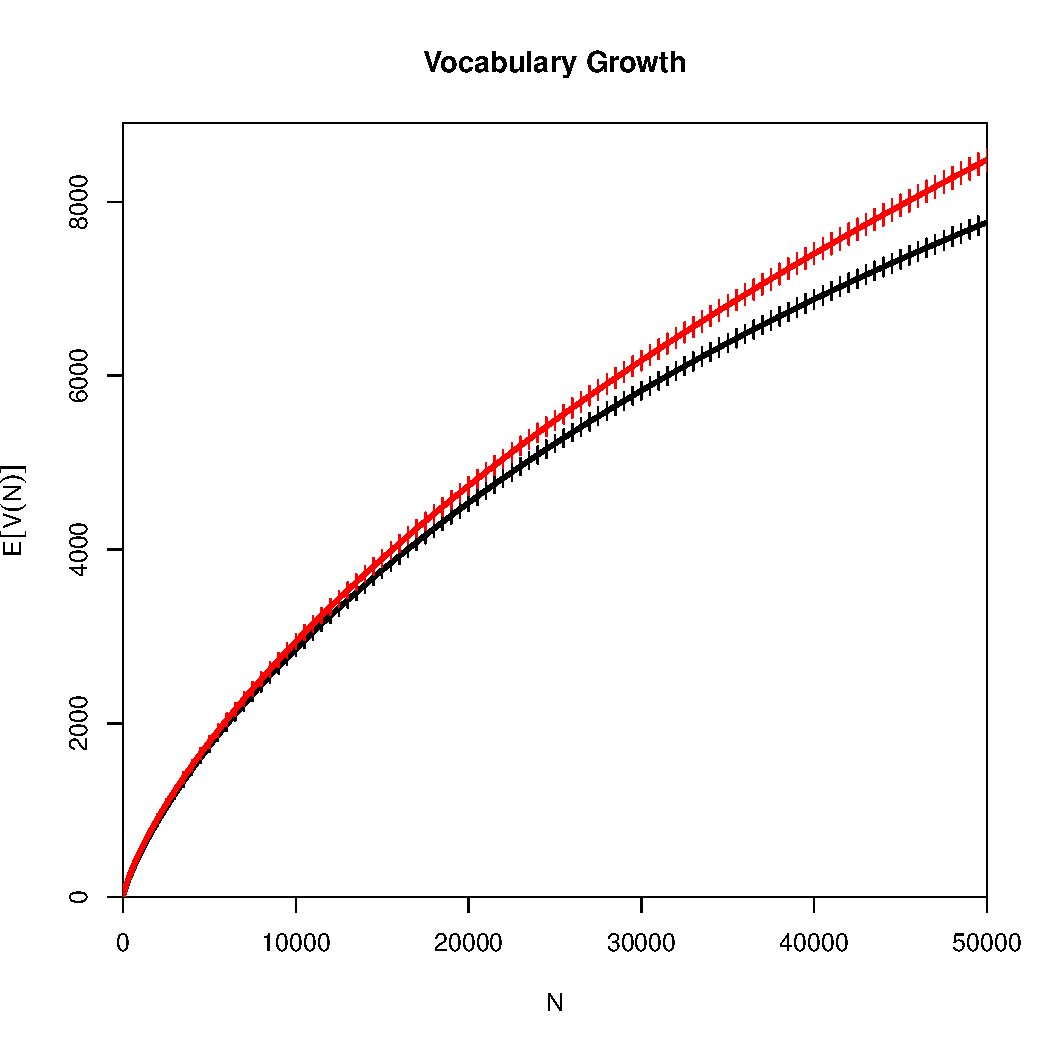
\includegraphics[width=250,height=250]{figure/Vgc-1} 

\end{knitrout}

read villa and vosters

Comparing some unique words from \textit{Trafalgar} and their first appearances in the Google N-gram data confirms this assumption.
Galdós redefines Spanish in a manner distinct from Isaacs, and defining Spanish was an intense debate throughout the mid-century.
The trans-atlantic polemic of refining Spanish grammar, orthography, and lexicon served as a symbol of socio-political struggles \cite[230]{Villa2015}.

The overwhelming amount of word differences between the two novels comes, as would be expected, from words with very low frequencies.
Around 880 words that occur only once in \textit{María} do not appear in \textit{Trafalgar}.
The number of unique hapax legomena in \textit{Trafalgar} is around 2850.
While part of the magnitude of difference is due to the fact that \textit{Trafalger} is considerably longer, the vocabulary is still impresively large.
The extrapolation of vocabulary curves seen in Figure 4 confirms what the hapax comparison shows.
A comparison of the ratio of hapax legomena to total tokens offers another means of comparing vocabulary richness across the corpora.

Figure 5 shows this ratio for all of the novels in the Gutenberg as well as the sub-corpora being examined here.

Figure 5:




As Laura Villa points out, the language ideology debate met with national policy in the 1800's when public teachers promoted a refined orthography in order to better facilitate reducing illiteracy.
This debate between educators and the Real Academia Española emerged simultaneous to the efforts in the Americas to establish and refine standards for Spanish in the Americas.
Domingo Sarmiento and Andres Bello proposed two different refinements of Spanish grammar and orthography.
At the same time other efforts to establish the American lexicon through cataloging the growing vernacular were widespread. 
The connection to state policy in the case of education in Spain was less over orthography than control over education policy that would shape the nation-forming public.
As Angel Rama points out in \textit{La ciudad letrada}, control over reading and writing had been a device of political control for centuries.
The centuries control over access to law and religion made the powerful connection between language and politics clear to the ruling classes.

Anderson points out that the importance of print vernaculars rose as unifying languages like Latin lost traction.
He notes that "the fall of Latin exemplified a larger process in which the sacred communities integrated by old sacred languages were gradually fragmented, pluralized, and territorialized \cite[19]{Anderson2006}. 
In Anderson's view, this \enquote{vernacularization}, coupling with expanding printing press capabilities, would have produced to many small inconsequential markets of \enquote{petty} proportions \cite[43]{Anderson2006}.
While Spanish in the Americas has not distinguished itself to the degree of the descendants of Latin, the nationalist drive to \enquote{associate language with territorial units} was nevertheless influential (43).
The struggle for distinction in the Americas was bottom-up, attempting to create regional identity within the ex-colonial linguistic superstrata.
In Spain, for the controlling class, the struggle was top down, fighting to maintain linguitic hegemony while regional language attempted to re-define themselves as central power declined.

In \textit{Trafalgar} this shows not only in Galdós' rich lexicon, but the source of his vocabulary as well. 
As Urey has mentioned the semantic re-purposing of terms, many military, by his characters provides one source.
In addition, Galdós uses many words whose usage reached its height in the 16th and 17th centuries.
The word \textit{rocín}, to cite one example, occurs 161 times in the 1600's in the \textit{Corpus del español} 11 in the 1700's, 51 in the 1800's and ceases to appear after that. 
Many other words, \textit{zampar, pimpollo}, follow a similar pattern.
The recycling of vocabulary was widespread with 19th century writers but more pertinent for defining regional vernaculars is the linguistic distinction this helped to create in literary vocabulary.
Using the same example, \textit{rocín} occurs 678 times in the \textit{Corpus Diacrónico del Español}, 91\% of those occurences being from Spain, 77\% \textit{pimpollo} occurs in documents from Spain. 
Even taking into consideration a skewed corpus composition, these two examples point to the possibility of a unique Spanish literary vocabulary.
There are 6660 words, not lemmatized, in \textit{Trafalgar} that do not occur in \textit{María}, which itself has only 2220 unique terms.
So while Isaacs gleaned much of his unique vocab from regional and indigenous vernacular, Galdós, and other peninsular author, turned to the archives.

%Rama p49 translation and semantics
While the importance of individual verbs over the course of the author's lexicon may not seem influential , it has a cumulative effect.
As Rama points out the educated elite throughout history has acted as translator of new and borrowed terms in order to determine what is admissable to \enquote{la norma cultural} \cite[50]{Rama2002}

The Spanish example stresses the awareness at the time of the identity forming power of language. The evolution of Gabriel as narrator throughout the \textit{Episodios nacionales}, as Urey points out, calls attention to the importance of writing and its ability to influence the reader. In \textit{María} this sentiment manifests itself in Isaacs meta-commentary on reading as it pertains to his characters personal qualities. This literary reflection of regional identification calls into question the validity of a comparison of nationalism and literature outside of its regional context. Consequently, looking for patterns in \enquote{Latin American} national literatures may yield results given common historical beginnings. However understanding individual contributions of literatures is more productive within their own frame of reference.



According to Rodríguez, Galdós had a distinct purpose for looking back in history which was to \enquote{reconstruct the past as an organic continuum} \cite[28]{Rodriguez1967}.
Distancing the narrator served to create a causal relationship between history and national development.


It could certainly be argued that much of the separation in vocab between \textit{Trafalgar} and other novels of the time is due the novel's wealth of nautical vocabulary.
While it is certainly a justifiable concern, I would argue that this nevertheless reflects the identity of  Galdós' audience.
Spain's internalization of its maritime history makes the vocabulary of \textit{Trafalgar} as important an identifying characteristic as the indeginisms of the Americas.
In \textit{Trafalgar} it helps locate the novel in a distant past, as by the time of Gabriel's present Spain has lost is global geopolitical might and internal conflict dominated.


Santiago Pérez Isasi maintains that literary national history in Spain cannot be discussed until one establishes a when the Spanish nation was born \cite[172]{Isasi2013}.
He goes on to distinguish between all encompassing definitions of national literature and those that define national literature with the language in which it is expressed, essentially equating all nationalism to linguistic nationalism. 
Those with a broader view, including peninsular Latin sources as the basis of Spanish nationalism, recognize a more geographic definition.
By highlighting national roots in non-Spanish languages some critics place an emphasis on the regional origins of what Isasi calls \enquote{Spanish-ness} \cite[173]{Isasi2013}.
This becomes especially problematic as some critics narrow the origins even further recognizing only the contributions identified with Castilian origins, denying any place in the creation of national identity made by Catalan, Galician or Basque.


Add Chiaramonte

According to Storm one of the most overlooked problems in Spanish national unity was the rise of political clientelism in the late nineteenth century \cite[147]{Storm2004}.
The situation worsened when Spains instituted alternating governance between two parties.
Relationships with local \textit{caciques} were critical, as Storm points out \enquote{concrete local and personal improvements thus depended on loyalty to a local boss, on clientele networks, and not on the functioning of a national state} \cite[148]{Storm2004}.

In the nineteenth century, according to Catholic reactionaries, \enquote{Spain should only be identified with Catholicism and the hierarchical social order that existed before foreign ideas had led the country astray}, a shift that they associated with the \enquote{plea for national sovereignty} \cite[149]{Storm2004}.


Gabriel reaches an epiphany midway through the novel when he proclaims:
\blockquote[{\cite[1127]{Galdos1882}}]{Por primera vez entonces percibí con completa claridad la idea de la patria [...] el patriotismo no era para mí más que el orgullo de pertenecer a aquella casta de matadores de moros. Pero en el momento que procedió al combate, comprendí todo lo que aquella divina palabra significaba, y la idea de nacionalidad se abrió paso en mi espíritu, [...] Me representé a mi país como una inmensa tierra poblada de gentes, todos fraternalmente unidos.}
His realization is a moment that strongly reinforces Iarocci's notion that the series narrates the protagonist's formation, framing it as sort of national \textit{bildungsroman}.
This view of nation as akin to personal development lacks sufficient exploration be Sommer in the American context.
Nevertheless, it could certainly be said that, off of the battlefield the characters of Efraín and Gabriel struggle with the challenges of love and family.

Jorge Coronado, in his examination of \textit{indigenismo} and the Andean region, asks of Anderson's definition of nation \enquote{what if the all-encompassing imagination of a community in a given geopolitical space is made not from a centralized locus of official power and through its organs, such as dominant print media, but rather from another marginalized position} \cite[12]{Coronado2009}?
Coronado examines mainly twentieth century \textit{indigenismo}, however the quandary of reconciling Anderson's definition with regional identity goes back to the beginning of independence in the Americas.
He asserts that regionalisms have been strong enough in the Andes to \enquote{mount a considerable response to the homogenization of a given geopolitical space proposed by nationalism} \cite[12]{Coronado2009}.
Throughout the Americas the question of defining who constituted \enquote{the real national subjects}, has existed since colonial times, with more marginalized groups gaining a voice as time progresses.
Spain was not immune to this fractured national paradigm, and by the end of the nineteenth century it will have made its way in Galdos' novels.

At the turn of the century Galdós admits an interest in the writing of Miguel de Unamuno, who claims to have influenced the later \textit{Episodios} as well as shared ideals on the question of regional autonomy \cite[291]{Kempen2007}.
In any event, these ideas do not directly enter into plot of the first novel, however it reinforces the idea that Galdós was keenly aware at the time of writing that the stakes for language and culture in Spain were high.
This helps to explain the focus on a losing battle, attempting to unite the various regional nations under the Spanish nation-state \cite{Kempen2007}.
The commentary on nation state is not entirely limited to matters of regional political divisions and military history.
Galdós also weaves into \textit{Trafalgar}, and to a much larger extent his other novels, allegories of family, love, and politics equal to those found in the Americas.

conclusion
Ngugi - returning the center

In historical investigations of linguistic phenomena recent scholarship has questioned top down qualitative divisions of diachronic periods. Stephen Gries is one linguist developing methods of bottom-up analysis, which while methodologically different from techiniques in digital literary analysis, theoretically relevant question of what degree of granularity is necessary is necessary when investigating an historical phenomenon? 

%\makeworkscited
\end{document}
